% Concise revision of the archived ICIP draft. Historical results, not new experiments.
\documentclass{article}
\usepackage{spconf,amsmath,amssymb,graphicx,booktabs,xcolor,url}
\usepackage{balance}
\graphicspath{{assets/}}
\renewcommand{\topfraction}{0.92}
\renewcommand{\dbltopfraction}{0.92}
\renewcommand{\textfraction}{0.08}
\title{OBSERVATION-ANCHORED LOW-FREQUENCY REPLACEMENT FOR ONE-STEP DIFFUSION SPATIOTEMPORAL FUSION}
\name{Anonymous Author(s)}
\address{Anonymous Affiliation}
\begin{document}
\ninept
\maketitle

\begin{abstract}
One-step diffusion spatiotemporal fusion (STF) reduces sampling cost but can retain low-frequency temporal bias.
We correct this bias by replacing the predicted low-frequency component with a target anchored to the reference images and coarse observation.
The operator fits no parameters and requires one network evaluation.
Across twenty inference-time variants, its archived LGC results improve RMSE over the uncorrected one-step output by 14.2\% on the stable split and 6.4\% on flood.
CIA reveals a transfer boundary: replacement improves test RMSE but degrades validation RMSE.
Fine/coarse change diagnostics ($a=0.544$, $R^2=0.278$) motivate the comparison with fitted calibration.
A nine-backbone study further exposes training trade-offs and a time-conditioned gate that collapses to a near-constant.
These exploratory results support observation anchoring while limiting claims of universal improvement.
\end{abstract}
\begin{keywords}
spatiotemporal fusion, diffusion models, low-frequency replacement, inference-time correction, remote sensing
\end{keywords}

\section{Introduction}
\label{sec:intro}
Diffusion STF reconstructs a fine image from two coarse/fine reference pairs and a coarse observation at the prediction date.
Recent models improve conditional generation~\cite{huang2024stfdiff,zhang2026sastf,zhu2026dpdiff}, but iterative sampling remains costly.
Reducing inference to one denoising call can leave temporal changes inconsistent with the coarse observation.

The dual-anchor protocol provides two reference pairs for inference-time correction.
One approach fits their fine/coarse relationship through regression, transport or distribution alignment.
Another directly anchors the prediction to observed change.
We examine when fitting helps and whether better training removes the need for correction.

Our contribution is a parameter-free low-frequency replacement, supported by a twenty-variant comparison and a nine-backbone training study.
The central evidence includes both LGC gains and the CIA validation failure.
The study therefore evaluates a bounded correction mechanism rather than establishing a universally best operator.

\section{Related Work}
\label{sec:related}
STFDiff introduces diffusion-based STF with a dual-stream predictor~\cite{huang2024stfdiff}.
SA-STF uses temporal alignment and semantic-adaptive fusion~\cite{zhang2026sastf}; DPDiff incorporates dual priors~\cite{zhu2026dpdiff}.
These methods change conditional generation.
Our operator instead corrects a frozen prediction using the observations already available under the same dual-anchor input protocol.
The comparison concerns fitted calibration and direct replacement, without additional inference-time fine images or parameter adaptation.

\section{Protocol and Operators}
\label{sec:method}
\subsection{Inputs and evaluation}
The inputs are $(F_p,C_p)$, $(F_n,C_n)$ and $C_t$; the target fine image $F_t$ is excluded from inference.
The frozen 7.49\,M-parameter backbone returns $x_1$ after one denoising call.
We use a Gaussian low-pass operator $\mathrm{LP}$ with $\sigma=2$ and a shared correction strength $\lambda=0.3$.
Reflectance is mapped to $[-1,1]$ for the model; RMSE is reported on $[0,1]$.

LGC contains 120 patches per split: stable validation uses 2005-02-14/03-02/04-03 and flood test uses 2004-12-28/2005-01-13/01-29.
CIA contributes 126 validation and 168 test patches.
The tables reproduce archived evaluations.
Checkpoint provenance, sampler settings and legacy metric differences remain under audit; these scores do not establish a matched-protocol external SOTA comparison.

\subsection{Replacement and fitted alternatives}
Calibration fits $\mathrm{LP}(F_n-F_p)\approx a\,\mathrm{LP}(C_n-C_p)+b$ from each sample's reference pairs.
For the preceding anchor, the target is
\begin{equation}
T_p=\mathrm{LP}(F_p)+a\,\mathrm{LP}(C_t-C_p)+b,
\label{eq:target}
\end{equation}
and the correction is
\begin{equation}
x_{\mathrm{out}}=x_1-\lambda\bigl(\mathrm{LP}(x_1)-T\bigr).
\label{eq:proj}
\end{equation}
The archived replacement uses $T=T_p$ and fixes $a=1,b=0$, removing the per-sample fit.
It adds a low-frequency correction while retaining the backbone prediction as the detail-bearing estimate.
Two-anchor variants use $T_n=\mathrm{LP}(F_n)+a\,\mathrm{LP}(C_t-C_n)-b$ and combine $T_p,T_n$ by averaging or inverse-variance weighting.

The twenty selected configurations cover OLS, TLS, Deming, Huber, ridge, change-weighted, inverse-variance, span-normalised and identity estimators.
They also examine Gaussian, Haar, guided and two-scale projections, distribution alignment, adaptive strengths and a two-step fixed point.
This is a selected configuration set, not the full estimator--projection Cartesian product.
Table~\ref{tab:operators} uses the shared $\lambda=0.3$; the broader configurations in Fig.~\ref{fig:gain} are distinguished from that fixed-strength comparison.

\begin{table*}[t]
\centering
\caption{Archived correction results on the frozen project checkpoint. RMSE on $[0,1]$, shared $\lambda=0.3$. A dash denotes an entry absent from the corresponding original table. Bold identifies the minimum in each column.}
\label{tab:operators}
\begin{tabular}{lcccc}
\toprule
 & \multicolumn{2}{c}{LGC, 120 patches/split} & \multicolumn{2}{c}{CIA, 126/168 patches}\\
\cmidrule(lr){2-3}\cmidrule(lr){4-5}
Method & Stable (val) & Flood (test) & Validation & Test\\
\midrule
Legacy 10-step sampler (10 NFE) & 0.02972 & 0.02161 & 0.02716 & 0.02777\\
Fixed-1 (1 NFE) & 0.02815 & 0.02053 & 0.02785 & 0.02741\\
Source-calibrated & 0.02577 & 0.01977 & -- & --\\
Per-sample OLS & 0.02810 & 0.01897 & 0.02776 & 0.02742\\
Huber & -- & -- & 0.02780 & 0.02722\\
Ridge-shrunk & 0.02787 & \textbf{0.01896} & 0.02769 & 0.02737\\
Gated calibration & 0.02724 & 0.01943 & \textbf{0.02709} & 0.02677\\
Low-frequency replacement & \textbf{0.02416} & 0.01921 & 0.02855 & \textbf{0.02659}\\
\bottomrule
\end{tabular}
\end{table*}

\subsection{Architecture and training variants}
\label{sec:arch}
The nine-backbone study includes base, three loss variants (low-frequency, high-frequency and band weighting), four architecture variants and delta supervision.
The architectures add explicit temporal differences ($+0.015$\,M parameters), a noise-time-conditioned sigmoid gate ($+0.016$\,M), multi-scale condition re-injection, or their combination.
Disabled branches were checked for zero output difference from the original predictor.

Delta supervision penalises deviations of $\mathrm{LP}(x_0)-\mathrm{LP}(F_p)$ from $0.54\,\mathrm{LP}(C_t-C_p)$.
The archived recipe specifies 1,200 patches from ten LGC triples, a nominal 40-epoch budget, Adam at $2\times10^{-4}$, 200-step warm-up, cosine decay and gradient clipping at 1.0.
Batch size is two in full precision, with fixed validation noise.
Actual checkpoint stages and independent evaluation settings must be distinguished from the nominal training budget.

\section{Results}
\label{sec:exp}
\subsection{LGC gains and the CIA boundary}
Replacement reduces LGC RMSE by 14.2\% on stable validation and 6.4\% on flood relative to Fixed-1 (Table~\ref{tab:operators}).
The archived patch-level Wilcoxon values are $p=2.1\times10^{-21}$ and $7.4\times10^{-17}$, with 99\% and 86\% of patches improving.
These are exploratory spatial comparisons, not independent-event or multiple-training-seed evidence.
OLS and ridge achieve lower flood RMSE, whereas replacement is strongest on the stable split.

On CIA, replacement improves test RMSE by 3.0\% over Fixed-1 but worsens validation RMSE by 2.5\%.
Gated calibration has the lowest validation error; replacement has the lowest test error.
The split dependence rules out the claim that one correction wins everywhere.

\begin{figure}[t]
\centering
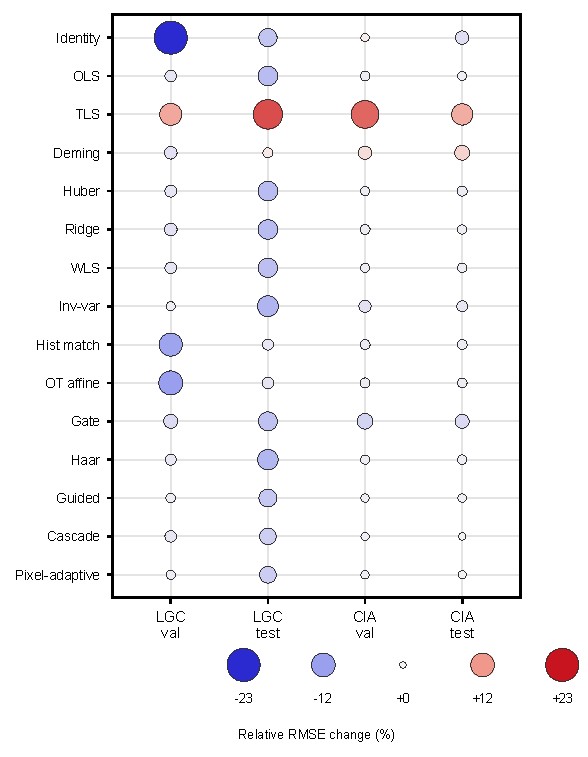
\includegraphics[width=0.94\linewidth]{fig2_gain_matrix_en.pdf}
\caption{Fifteen displayed correction variants across four splits. Blue denotes improvement and red degradation. These broader configurations include split-dependent strengths and are distinct from the fixed-strength table.}
\label{fig:gain}
\end{figure}

\subsection{What the calibration diagnostics explain}
The stable-split fine/coarse change fit gives $a=0.544$ and $R^2=0.278$; the prediction fit gives $a=0.473$ and $R^2=0.202$.
The backbone already reproduces much of the attenuated linear response.
Weak residual predictability makes additional per-sample fitting vulnerable to variance, motivating direct observation anchoring.
These correlations support the diagnosis but do not establish an irreducible information limit or a causal sensor explanation.

Figure~\ref{fig:gain} shows that correction benefits change with the regime and configuration.
On the retrained backbone, the stable-split comparison reports OLS degradation of 9.6\% and replacement improvement of 13.5\%.
Thus calibration performance depends on both the observations and the underlying prediction.

\subsection{Training does not remove the trade-off}
\begin{table}[t]
\centering
\caption{Nine-backbone evaluation. RMSE is on $[0,1]$; SSIM retains the legacy $[-1,1]$ input domain and is not mixed with the corrected metric protocol.}
\label{tab:backbones}
\setlength{\tabcolsep}{2.5pt}
\begin{tabular}{lcccc}
\toprule
 & \multicolumn{2}{c}{Stable (val)} & \multicolumn{2}{c}{Flood (test)}\\
\cmidrule(lr){2-3}\cmidrule(lr){4-5}
Backbone & RMSE & SSIM & RMSE & SSIM\\
\midrule
Base & \textbf{0.02329} & 0.8918 & 0.02160 & 0.8683\\
+LF loss & 0.02448 & 0.8895 & 0.02104 & 0.8727\\
+HF loss & 0.02415 & 0.8959 & 0.02083 & 0.8762\\
+Band weights & 0.02424 & 0.8913 & 0.02122 & 0.8702\\
+Delta supervision & 0.02491 & 0.8434 & 0.02450 & 0.8181\\
Arch: full & 0.02602 & 0.8932 & 0.02334 & 0.8722\\
Arch: delta & 0.02522 & 0.8917 & \textbf{0.02063} & 0.8743\\
Arch: gate & 0.02488 & 0.8922 & 0.02123 & 0.8755\\
Arch: reinject & 0.02559 & 0.8885 & 0.02160 & 0.8722\\
\bottomrule
\end{tabular}
\end{table}

No training variant improves both LGC splits (Table~\ref{tab:backbones}).
Explicit differences achieve the lowest flood RMSE, but all variants worsen stable RMSE.
Delta supervision improves the internal fixed-noise validation trajectory yet degrades the independently reported scores.
This discrepancy makes validation-noise sensitivity a necessary control.

The trained gate remains near $g(t)=0.622$ across all hundred noise levels.
The intended time-dependent trust mechanism therefore behaves like constant rescaling.
This is a concrete negative result, rather than evidence that reliability cannot be learned by any training objective.

\begin{figure}[t]
\centering
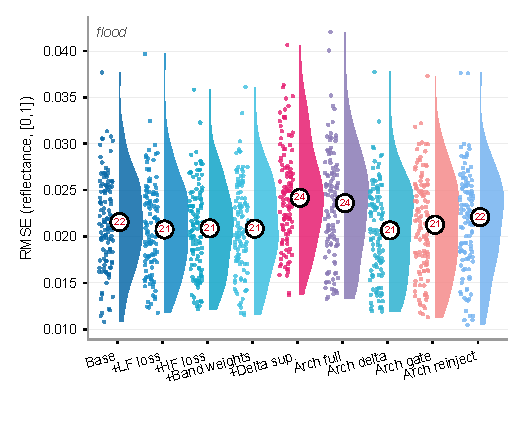
\includegraphics[width=\linewidth]{fig1_raincloud_en.pdf}
\caption{Flood-split patch RMSE across nine backbones: dots show patches, half-violins show density and circles mark medians ($\times10^{-3}$). These are model variants, not repeated training seeds.}
\label{fig:rain}
\end{figure}

\subsection{Combined system and computation}
\begin{table}[t]
\centering
\caption{System comparison, RMSE on $[0,1]$. The combined system uses the retrained backbone and replacement at $\lambda=0.3$.}
\label{tab:system}
\setlength{\tabcolsep}{2.5pt}
\begin{tabular}{lcccc}
\toprule
 & \multicolumn{2}{c}{LGC} & \multicolumn{2}{c}{CIA}\\
\cmidrule(lr){2-3}\cmidrule(lr){4-5}
Method & Stable & Flood & Val & Test\\
\midrule
Legacy 10-step & 0.02972 & 0.02161 & \textbf{0.02716} & 0.02777\\
Fixed-1 & 0.02815 & 0.02053 & 0.02785 & 0.02741\\
Combined & \textbf{0.02014} & \textbf{0.02044} & 0.02846 & \textbf{0.02664}\\
\bottomrule
\end{tabular}
\end{table}

The combined system reaches 0.02014 on LGC stable, 32.2\% below the archived ten-step score and 16.6\% below replacement alone.
It also improves on that ten-step score for flood and CIA test, but worsens CIA validation (Table~\ref{tab:system}).
Replacement alone remains better than the combined system on flood and CIA test.
Retraining therefore adds a stable-split gain rather than a uniform improvement.

Replacement uses one network evaluation (NFE), versus ten for the iterative baseline, plus separable filtering.
The archived CPU measurements are 0.93\,s versus 4.65\,s per patch, approximately a fivefold measured speed-up.
Tenfold fewer network calls should not be equated with a tenfold wall-clock speed-up.

\balance
\section{Conclusion}
\label{sec:concl}
Observation-anchored replacement offers a simple correction for one-step diffusion STF.
The archived comparisons show substantial LGC gains, a CIA validation failure, and training variants that do not resolve both LGC regimes.
The linear-change diagnostics and gate collapse help delimit the mechanism.
Matched sampler settings, corrected metrics, multiple training seeds and common-protocol external comparisons remain necessary for final performance claims.

\bibliographystyle{IEEEbib}
\bibliography{refs}
\end{document}
